\clearpage
\section{Numerical sanity checks}
\label{sec:numerical-sanity}

We examine the non-spikiness condition in
\Cref{assumption-main-coupled-particle-regularity}(iii) and the behavior of
adaptive PWGF with each system making its own perturbation decisions.
Following \citet[Algorithm~1]{yamamoto2025hessianguided}, the trigger uses the
\(L^2\) norm of the gradient under that system's current distribution.
We use a smooth matrix-factorization model, separate from the spherical model
of \Cref{sec:matrix-factorization}.

\subsection{Model and population--particle comparison}
\label{subsec:numerical-model}

\noindent\textbf{Objective and initial law.}
A particle is a matrix \(W\in\mathbb R^{32\times2}\), identified with
\(\mathbb R^{64}\) by row-major vectorization; matrix norms below are
Frobenius norms. With entrywise \(\tanh\), set
\begin{equation}
 F(\nu)=f(A_\nu),\qquad
 f(A)=\frac14\|AA^\top-M_*\|_F^2,\qquad
 A_\nu=\int\tanh(W)\,\nu(dW).
 \label{eq:numerical-objective}
\end{equation}
Here \(M_*=u_1u_1^\top+\tfrac12u_2u_2^\top\), where
\((u_1)_a=1/\sqrt{32}\) and
\((u_2)_a=(-1)^{a-1}/\sqrt{32}\) for \(1\le a\le32\).
Thus the objective factorizes the mean transformed particle.
Generate \(2^{14}\) matrices \(Z_a\) with independent standard normal entries
once (seed 20260925), and fix the realized population law
\[
 P_a(0-)=Z_a,\quad P_{a+2^{14}}(0-)=-Z_a,\qquad
 \mu_{0-}=2^{-15}\sum_{a=1}^{2^{14}}(\delta_{Z_a}+\delta_{-Z_a}).
\]
The notation \(0-\) denotes initialization before a possible jump at \(t=0\).
For each of three trials, sample labels \(I_i\) independently and uniformly
from \(\{1,\ldots,2^{15}\}\), independently of the population innovations, and
set \(X_{0-}^i=P_{I_i}(0-)\) before that jump. We use
\(N\in\{2048,4096,8192,16384,32768\}\), with nested label prefixes within each
trial. Sampling is with replacement, including at \(N=32768\).

\noindent\textbf{Continuous dynamics.}
The specified population has 32768 atoms, all of which are evolved; its
integrals are full atom averages. The empirical system uses only its sampled
particles:
\[
 \mu_t=2^{-15}\sum_{a=1}^{2^{15}}\delta_{P_a(t)},\qquad
 \widehat\mu_t^N=\frac1N\sum_{i=1}^N\delta_{X_t^i},\qquad
 Y_t^i=P_{I_i}(t).
\]
The ODEs and their shared velocity formula are
\begin{equation}
\begin{aligned}
 &\dot P_a(t)=-\nabla_WF(\mu_t,P_a(t)),\qquad
 \dot X_t^i=-\nabla_WF(\widehat\mu_t^N,X_t^i),\\
 &-\nabla_WF(\nu,W)=-(1-\tanh^2W)\odot
             [(A_\nu A_\nu^\top-M_*)A_\nu],
\end{aligned}
\label{eq:numerical-flow}
\end{equation}
where \(\odot\) is entrywise multiplication. In particular, for
\(F_N(\mathbf X)=F(\widehat\mu^N)\), the particle velocity is
\(-N\nabla_{X^i}F_N\). We integrate both systems by RK4; the population is
a fixed discrete measure, not a Monte Carlo approximation to a continuous law.

\noindent\textbf{Gaussian jumps.}
For a matrix \(W\), write
\(J_W=\operatorname{diag}(\operatorname{vec}(1-\tanh^2W))\) and
\(S_\nu=\int J_U^2\,\nu(dU)\).
Since \(\nabla f(A)=(AA^\top-M_*)A\), differentiation in a matrix direction
\(B\in\mathbb R^{32\times2}\) gives
\(\mathrm D(\nabla f)(A)[B]=(BA^\top+AB^\top)A+(AA^\top-M_*)B\).
Thus the symmetric matrix \(L_A\in\mathbb R^{64\times64}\) representing the
Hessian of \(f\) satisfies
\[
 L_A\operatorname{vec}(B)=\operatorname{vec}\bigl(
 (AA^\top-M_*)B+B(A^\top A)+AB^\top A\bigr).
\]
Thus the integral Hessian and its Gaussian covariance from
\Cref{subsec:population-pwgf} are
\begin{equation}
 \nabla_W^2F(\nu;W,V)=J_WL_{A_\nu}J_V,\qquad
 K_\nu(W,V)=J_WL_{A_\nu}S_\nu L_{A_\nu}^\top J_V.
 \label{eq:numerical-covariance}
\end{equation}
Since \(\operatorname{vec}(\mathrm D\tanh(V)[B])=J_V\operatorname{vec}(B)\),
the chain rule in \cref{eq:numerical-flow} yields the first identity.
The kernel composition in \Cref{subsec:population-pwgf} gives
\(K_\nu(W,V)=\int (J_WL_{A_\nu}J_U)(J_UL_{A_\nu}J_V)\,\nu(dU)
=J_WL_{A_\nu}S_\nu L_{A_\nu}J_V\), where
\(S_\nu=\int J_U^2\,\nu(dU)\) and \(L_{A_\nu}=L_{A_\nu}^\top\).
A draw of the field is
\(\operatorname{vec}(\xi_\nu(W))=J_WL_{A_\nu}S_\nu^{1/2}z\),
using one \(z\sim\mathcal N(0,I_{64})\) for all \(W\); its covariance is
\(K_\nu(W,V)\) because
\(S_\nu^{1/2}\mathbb E[zz^\top]S_\nu^{1/2}=S_\nu\).
The Gaussian rank is at most 64 even without finite support.
At their respective trigger times, the population and particle jumps have
marginal laws
\begin{equation}
\begin{aligned}
 P_a^+&=P_a^-+\eta\xi_{\mu^-}(P_a^-),\\
 \operatorname{vec}(X^{i,+}-X^{i,-})
 &=\frac\eta{\sqrt N}\sum_{j=1}^N
 \nabla_W^2F(\widehat\mu^{N,-};X^{i,-},X^{j,-})g_j,
 \qquad g_j\overset{\mathrm{iid}}\sim\mathcal N(0,I_{64}).
\end{aligned}
\label{eq:numerical-jumps}
\end{equation}
The implementation uses equivalent 64-dimensional factors.
The population path is generated first. Its \(j\)-th innovation is coupled,
by covariance-factor alignment with independent Gaussian completion, to the
empirical system's \(j\)-th attempt. An unmatched empirical attempt uses a
fresh independent field with its empirical covariance. This coupling uses
attempt index, not common physical time; the reference particles do not enter
the controller.

\subsection{Adaptive controller and recorded diagnostics}
\label{subsec:numerical-diagnostics}

Each system follows the gradient-trigger, wait, and decrease-test pattern of
\citet[Algorithm~1]{yamamoto2025hessianguided}. The controller acts separately
for the population and each particle system:
\begin{enumerate}
\item \textbf{Inspect and perturb.}
At \(t=0,0.1,\ldots,99.9\), if the system has not stopped and no waiting
window is active, test its pre-jump state using
\[
\begin{aligned}
\text{population:}\quad &
 \left(2^{-15}\sum_{a=1}^{2^{15}}
 \|\nabla_WF(\mu_{t-},P_a(t-))\|_F^2\right)^{1/2}\le0.01,\\
\text{particles:}\quad &
 \left(\frac1N\sum_{i=1}^N
 \|\nabla_WF(\widehat\mu_{t-}^N,X_{t-}^i)\|_F^2\right)^{1/2}\le0.01.
\end{aligned}
\]
These are the respective \(L^2\)-gradient norms, evaluated from
\cref{eq:numerical-flow}; each system uses its own measure in both the gradient
and the average. When its inequality holds, save the pre-jump measure and
apply the corresponding jump in \cref{eq:numerical-jumps} with \(\eta=0.2\).
Otherwise, continue the flow to the next inspection time.
\item \textbf{Wait and test the decrease.}
After a jump at \(s\), evolve for 10 time units without another jump, then
compare the objective with the saved pre-jump value:
\[
\begin{cases}
 \text{resume inspection at the next grid tick},
   &F(\nu_{s-})-F(\nu_{s+10})>0.001,\\
 \text{stop and return }\nu_{s-},
   &F(\nu_{s-})-F(\nu_{s+10})\le0.001.
\end{cases}
\]
Here \(\nu\) is the measure of the system being tested. A passed decrease test
does not trigger another jump at \(s+10\); inspection resumes at \(s+10.1\)
if time remains before the cap of 100. The returned candidate \(\nu_{s-}\)
is distinct from the executed state \(\nu_{s+10}\).
\end{enumerate}

\begin{center}
\begin{tabular}{@{}lclc@{}}
\toprule
Parameter & Value & Parameter & Value\\
\midrule
Jump amplitude \(\eta\) & 0.2 & Gradient threshold & 0.01\\
Waiting time & 10 & Decrease threshold & 0.001\\
RK4 step & 0.05 & Inspection interval & 0.1\\
Time cap & 100 & Trials & 3\\
\bottomrule
\end{tabular}
\end{center}

\noindent\textbf{Non-spikiness.}
At common physical times while both systems remain active, we compute the
paired error from \Cref{subsec:tracking-metric} and its cubic ratio:
\begin{equation}
 r_t=\left(\frac1N\sum_i\|X_t^i-Y_t^i\|_F^2\right)^{1/2},\qquad
 s_t=\frac{N^{-1}\sum_i\|X_t^i-Y_t^i\|_F^3}{r_t^3}.
 \label{eq:numerical-spikiness}
\end{equation}
We record inspection times and both sides of each jump, and omit \(s_t\)
when \(r_t\le10^{-12}\max\{1,(N^{-1}\sum_i\|Y_t^i\|_F^2)^{1/2}\}\).
Across all 15 conditions, the largest recorded ratio is 1.017416.
\Cref{fig:numerical-spikiness} therefore supports non-spiky paired errors in
these runs: the empirical analogue of
\Cref{assumption-main-coupled-particle-regularity}(iii) is close to one at
recorded times. This is not a bound over all continuous times or random paths.

\begin{figure}[!ht]
\centering
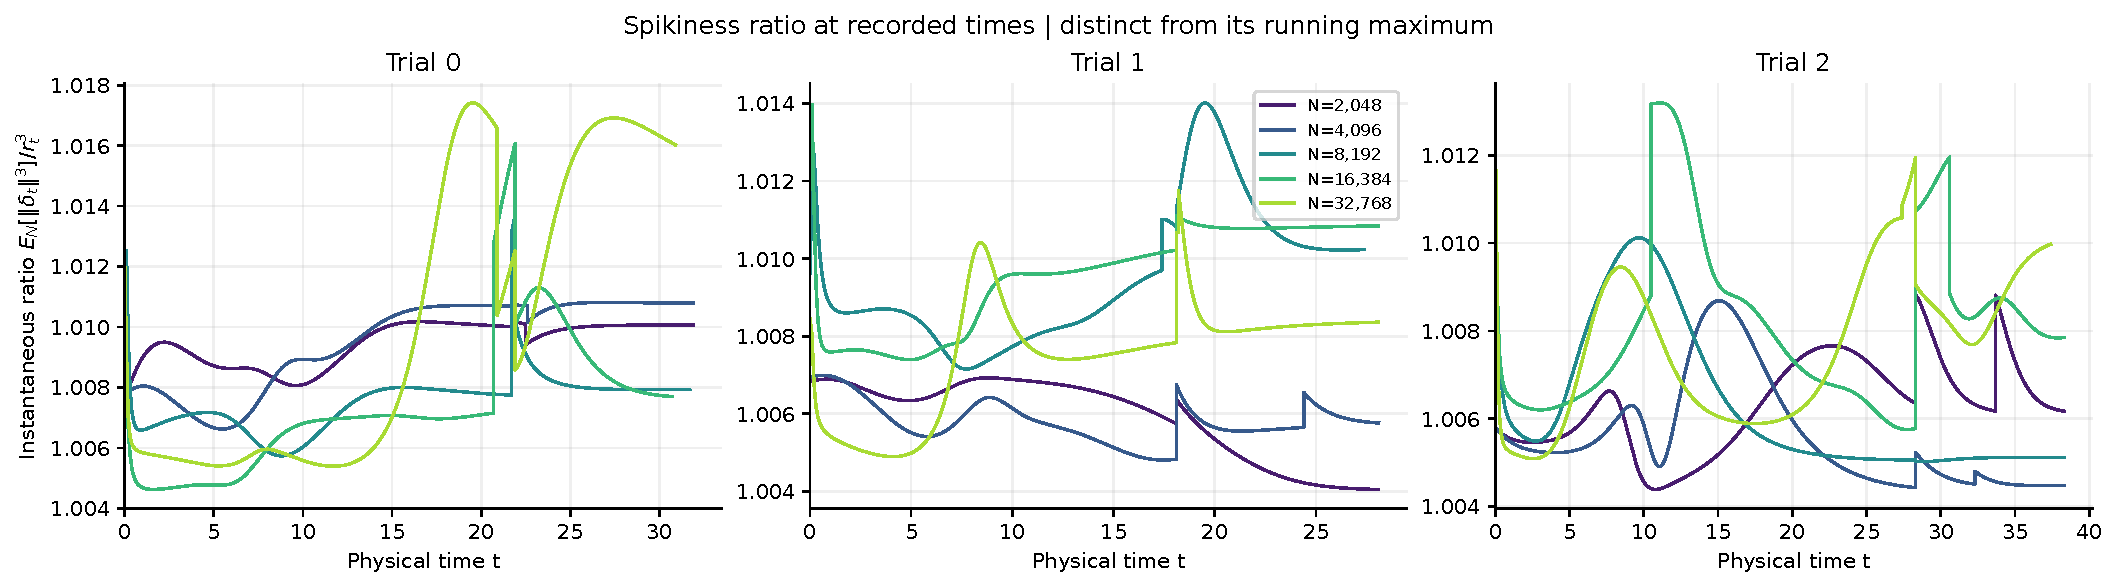
\includegraphics[width=\linewidth]{appendix_numerical/figures/adaptive_K32768_instantaneous_spikiness_20260925-220740JST_e1f6acdcbae6.pdf}
\caption{The instantaneous cubic ratio \(s_t\) in
\cref{eq:numerical-spikiness}, with all three trials and five particle counts.
Curves end when either system stops; near-zero denominators are omitted.
The ratio measures the distribution of paired errors, not particle positions.}
\label{fig:numerical-spikiness}
\end{figure}

\noindent\textbf{Adaptive schedules.}
All 15 particle systems and three population paths stopped before the cap;
the empirical returned objectives ranged from \(1.12\times10^{-4}\) to
\(1.41\times10^{-4}\).
\Cref{fig:numerical-schedules} illustrates autonomous decisions based on each
system's own \(L^2\)-gradient test: all \(N=2048,4096\) systems skip the
population's initial jump, and trial 2 at \(N=16384\) makes a third attempt
without a population counterpart. The resulting differences in physical jump
times can produce temporary same-time discrepancies: at \(N=32768\), recorded
peaks of \(r_t\) range from 0.584 to 0.601. Discrepancies can be much larger
at smaller \(N\) and are not monotone in \(N\), despite the near-unit spikiness
ratios. These diagnostics complement \Cref{theorem-main-r_t}; its guarantee
remains for a prescribed common schedule.

\begin{figure}[!ht]
\centering
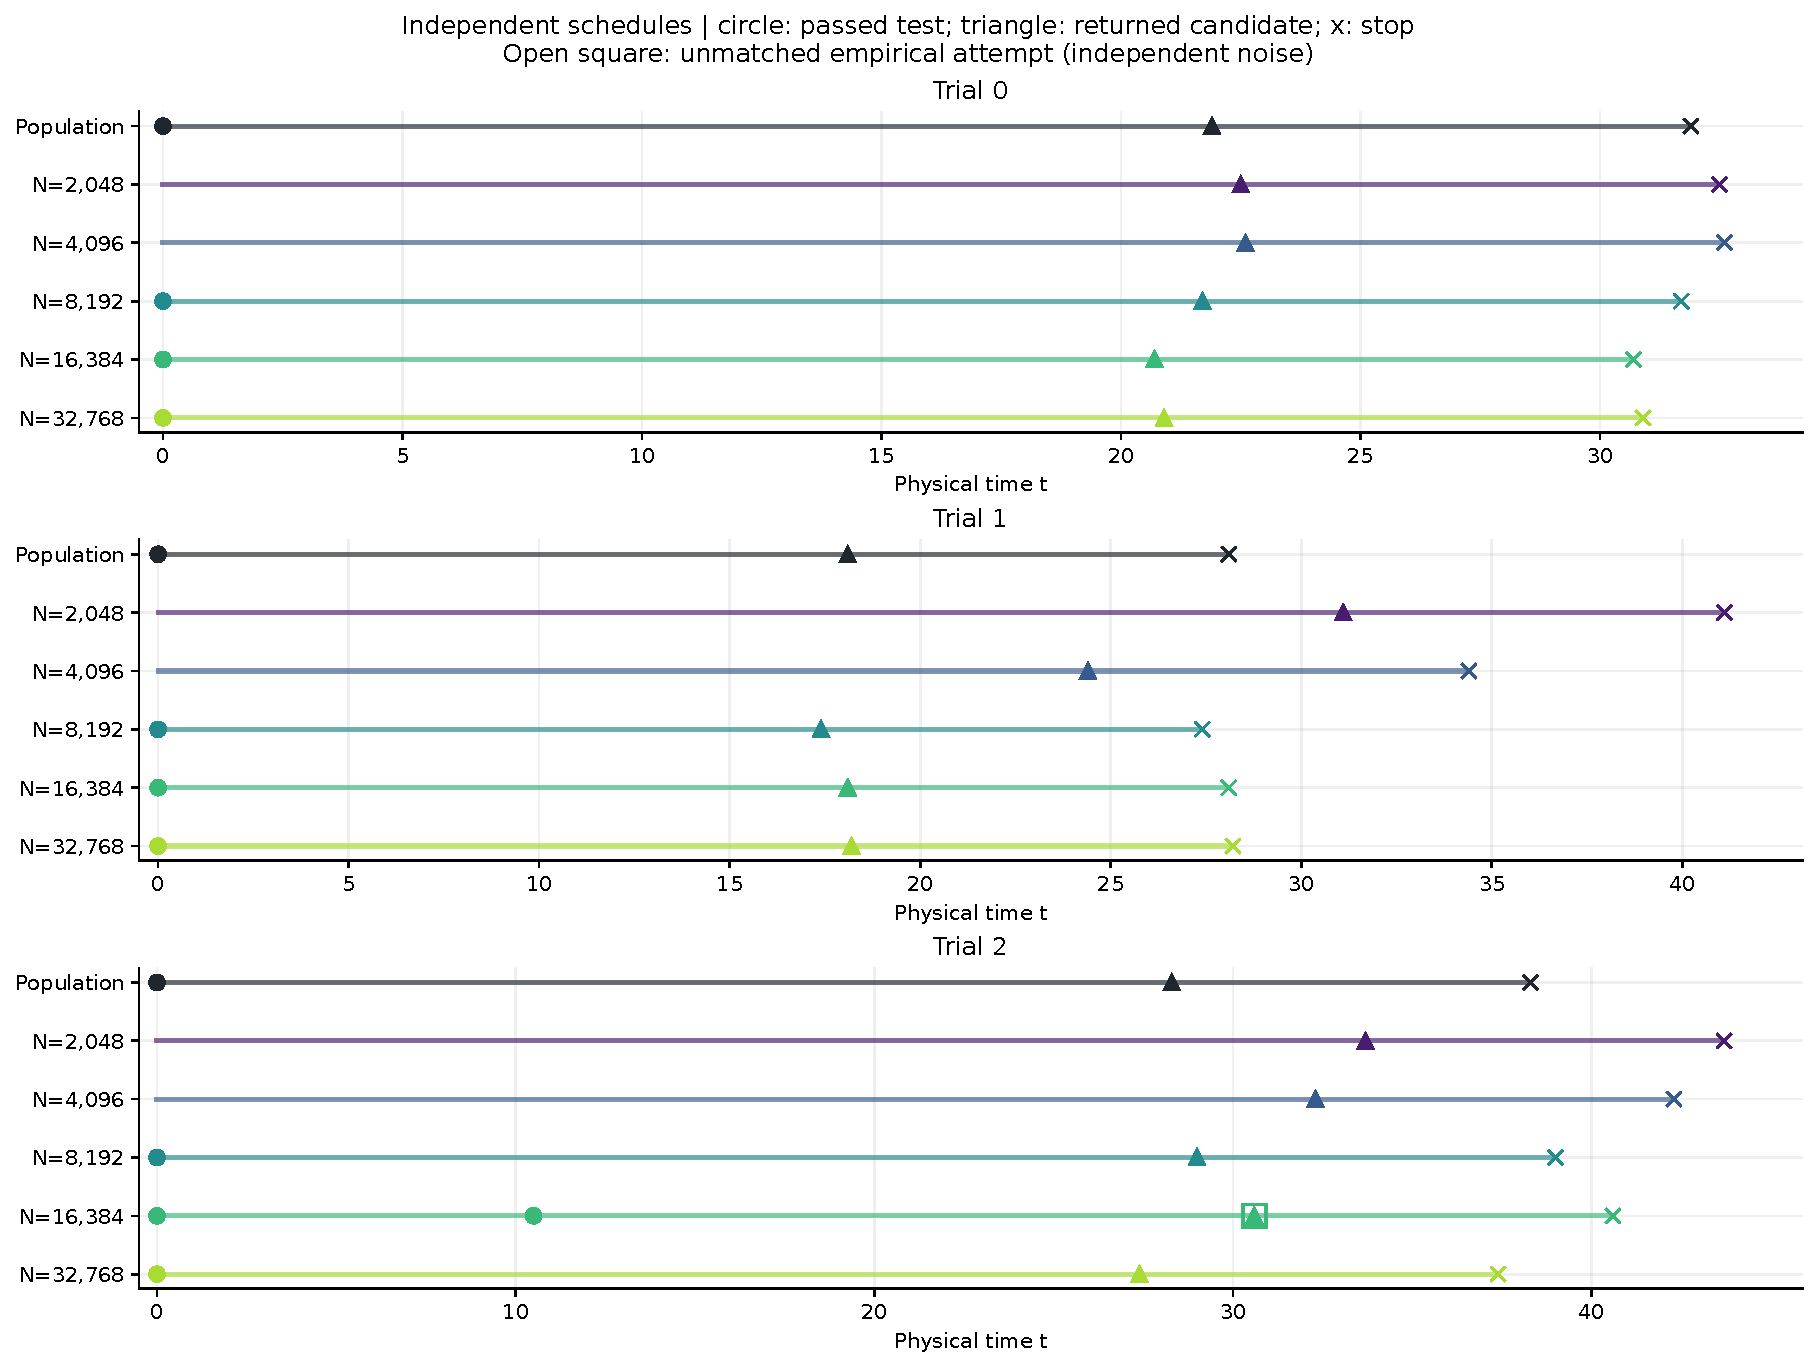
\includegraphics[width=\linewidth]{appendix_numerical/figures/adaptive_K32768_schedules_20260925-220741JST_41bda0385c70.pdf}
\caption{Independently chosen adaptive schedules, showing every system.
Circles mark jumps whose decrease test passes; triangles mark the saved
pre-jump candidates returned after a failed test; crosses mark stopping times.
The open square marks an unmatched empirical attempt. Coupling by attempt
index does not force jump times to coincide.}
\label{fig:numerical-schedules}
\end{figure}

\noindent\textbf{Numerical checks and reproduction.}
Halving the RK4 step preserved all event times and counts; halving the
inspection interval preserved counts but shifted some event times by 0.05.
The latter changed individual returned objectives by up to
\(4.89\times10^{-6}\), so small objective gaps are not used to infer a rate.
Code, configurations, exact seeds, and archived scalar records are provided
in the accompanying anonymous supplementary package.

\clearpage
\subsection{Paired trajectories and objective values}
\label{subsec:numerical-tracking}

\Cref{fig:numerical-tracking} shows the paired error \(r_t\) from
\cref{eq:numerical-spikiness} and the objective gap
\(\lvert F(\widehat\mu_t^N)-F(\mu_t)\rvert\) at the same physical time.
\Cref{fig:numerical-objectives} shows the objective values themselves, using
\cref{eq:numerical-objective}, until each system stops. Together they show
particle discrepancies and optimization progress under separately triggered
jumps.

\begin{figure}[!ht]
\centering
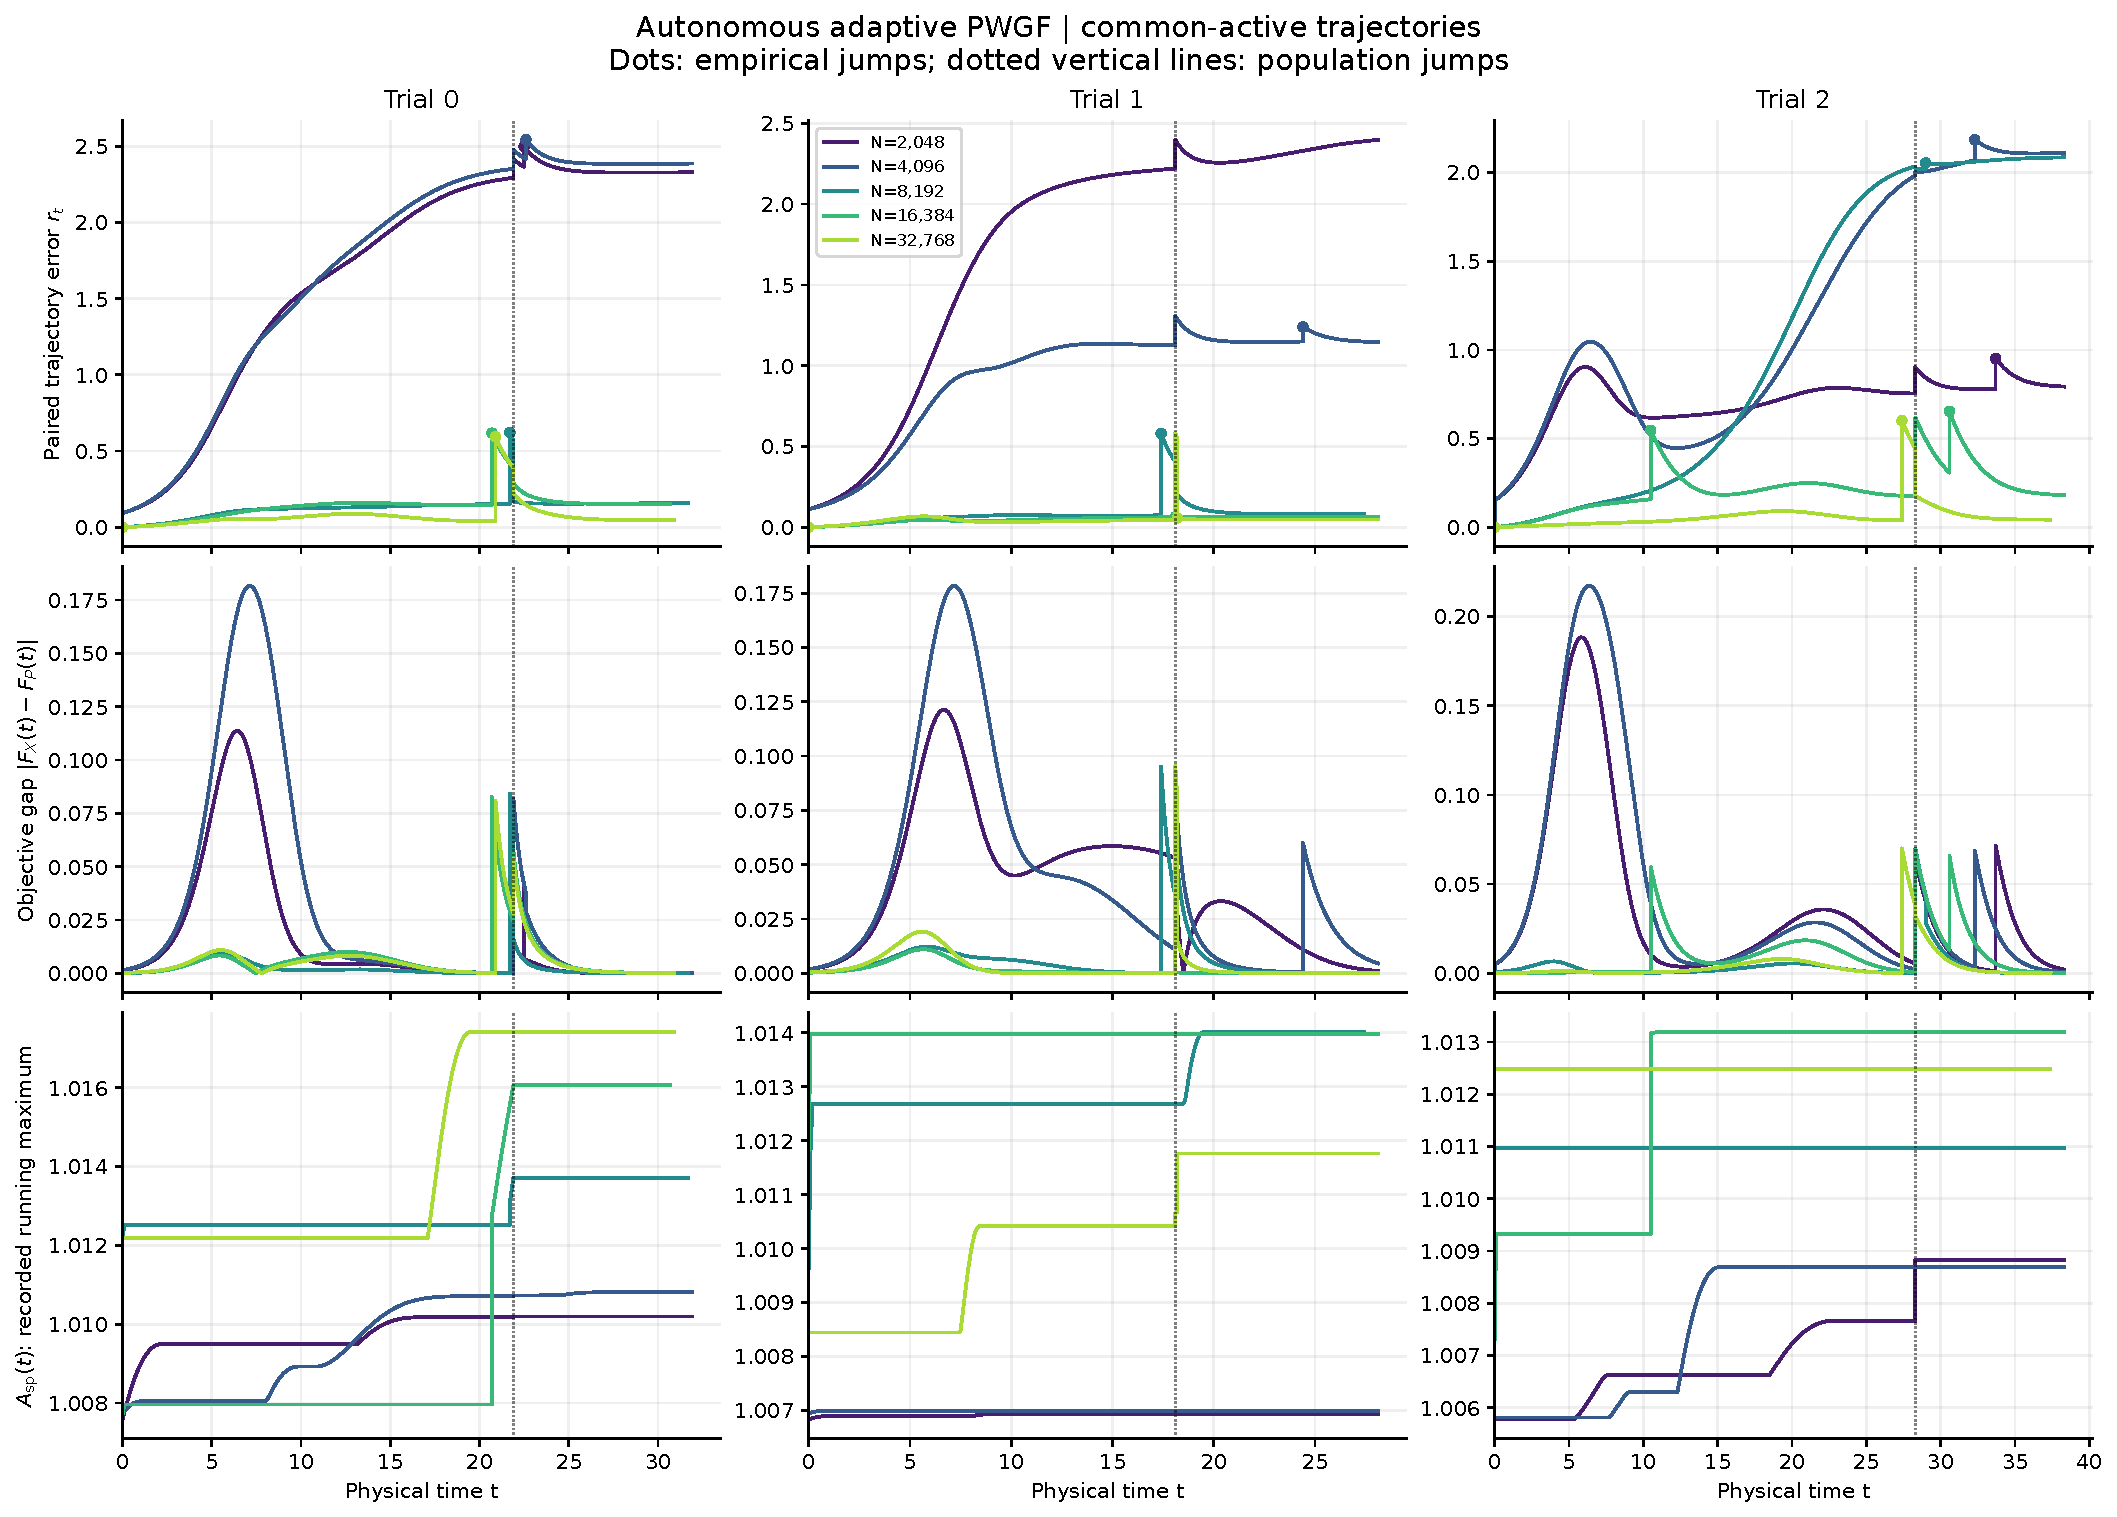
\includegraphics[width=\linewidth]{appendix_numerical/figures/adaptive_K32768_time_tracking_20260925-220738JST_402967415f7c.pdf}
\caption{Common-time diagnostics for all 15 conditions, with one column per
trial. Top: paired RMS error \(r_t\).
Middle: \(\lvert F_X(t)-F_P(t)\rvert\), where
\(F_X(t)=F(\widehat\mu_t^N)\) and \(F_P(t)=F(\mu_t)\).
Bottom: the running maximum of the recorded ratio \(s_t\), labeled
\(A_{\rm sp}(t)\), rather than its instantaneous value in
\cref{fig:numerical-spikiness}. Dots in the top row mark empirical jumps;
dotted vertical lines mark population jumps. Curves end when either system
stops; vertical segments connect recorded pre/post-jump values.}
\label{fig:numerical-tracking}
\end{figure}

\begin{figure}[!ht]
\centering
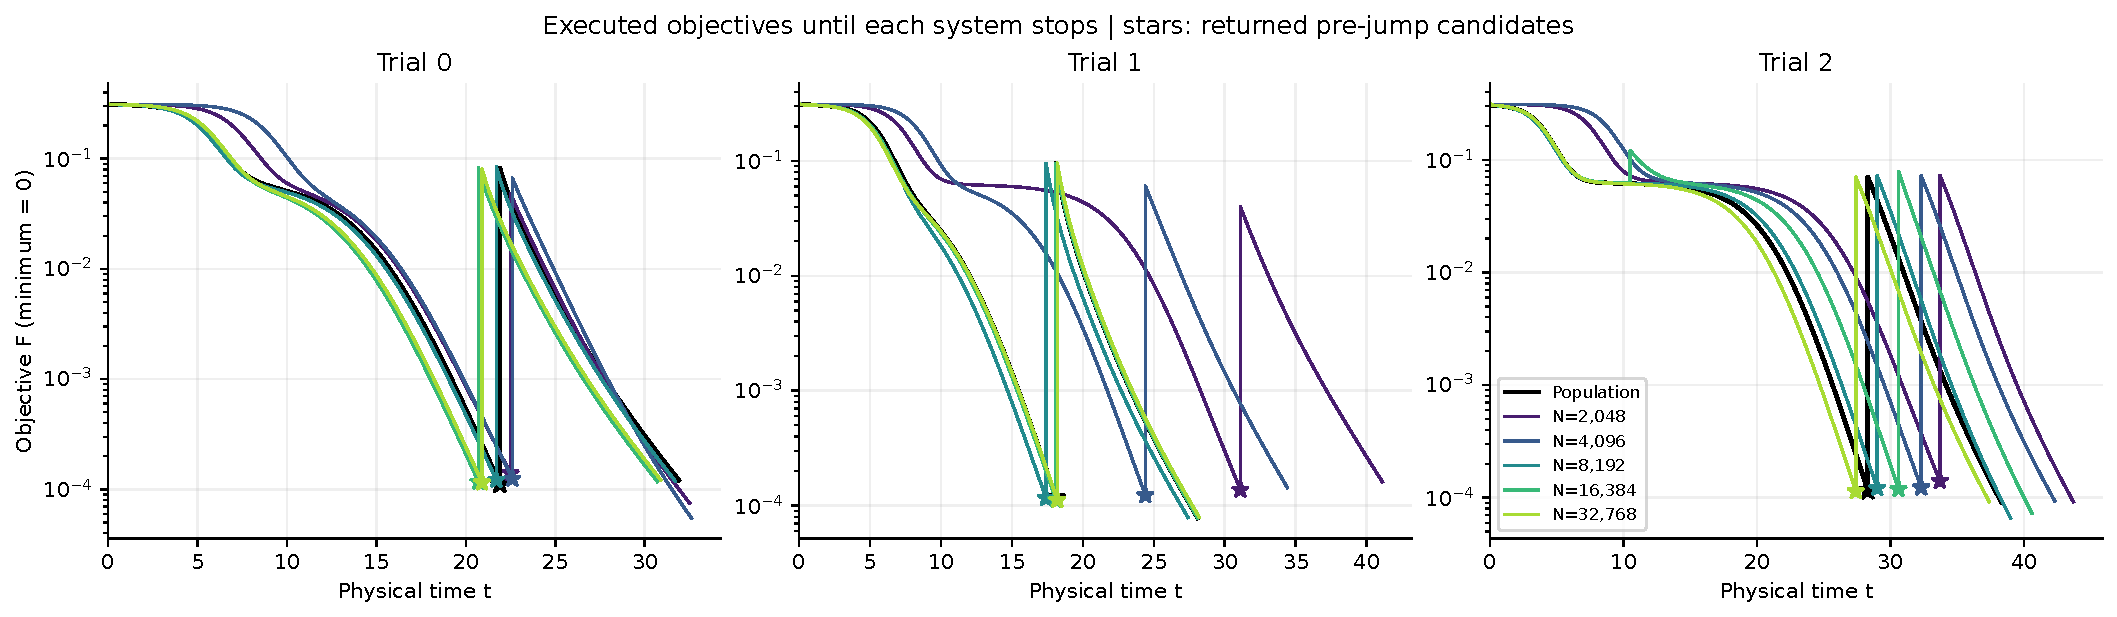
\includegraphics[width=\linewidth]{appendix_numerical/figures/adaptive_K32768_objectives_20260925-220741JST_f5f6c2a2d261.pdf}
\caption{Objective values \(F(\mu_t)\) (black) and
\(F(\widehat\mu_t^N)\) (colored) for every trial and particle count.
Each curve continues to that system's own stopping time. Stars mark the
saved pre-jump candidates at their candidate times, rather than the final
executed states. The minimum of \cref{eq:numerical-objective} is zero.}
\label{fig:numerical-objectives}
\end{figure}
